\documentclass[11pt]{beamer}

% Theme and packages
\usetheme{Madrid}
\usecolortheme{default}
\useoutertheme{default} % removes bottom bars
\setbeamertemplate{footline}{} % removes footer bar
\setbeamertemplate{navigation symbols}{} % removes navigation icons

\usepackage{amsmath, amssymb, amsfonts}
\usepackage{tikz}
\usetikzlibrary{shapes.geometric, arrows}
\usepackage{fancyvrb}

\usepackage{pgfplots}

% Flowchart styles
\tikzstyle{startstop} = [rectangle, rounded corners, minimum width=3cm, minimum height=1cm,text centered, draw=black, fill=red!30]
\tikzstyle{process} = [rectangle, minimum width=3cm, minimum height=1cm, text centered, draw=black, fill=blue!20]
\tikzstyle{decision} = [diamond, aspect=2, text centered, minimum width=3cm, draw=black, fill=green!20]
\tikzstyle{arrow} = [thick,->,>=stealth]

% Title information
\title[Factorization of Ideals]{Factorization of Algebraic Ideals and Its Applications}
\author{Brent Baccala}
\institute{\tt cosine@freesoft.org}
\date{October 1, 2025}

\begin{document}

%----------------------------------
% Title Slide
%----------------------------------
\begin{frame}
  \titlepage
\begin{block}{Abstract}
\tiny
Decomposing an ideal into an intersection of prime or primary ideals is a fundamental operation in commutative algebra, one that should be known to all math students for its utility in simplifying systems of polynomial equations.  Various algorithms have been proposed and implemented for ideal factorization, including the method of characteristic sets and the GTZ algorithm.  In this talk, I'll describe some of these methods, illustrate them with one or two examples, and explain their application to solving polynomial and differential equations.
\end{block}

\end{frame}

%----------------------------------
\begin{frame}{Motivation}
\begin{itemize}
  \item Ideal decomposition simplifies systems of polynomial equations.
  \item Differential equations can also be solved this way.
\end{itemize}
\end{frame}

%----------------------------------
\begin{frame}{Background: Ideals in Commutative Algebra}
%\begin{columns}
%\column{0.55\textwidth}
\begin{itemize}
  \item An \textbf{ideal} $I \subset R$ is a subset closed under addition and multiplication by ring elements.
  \item \textbf{Prime ideal:} if $ab \in P$, then $a \in P$ or $b \in P$.
  \item \textbf{Primary ideal:} if $ab \in Q$, then $a \in Q$ or $b^n \in Q$.
  \item \textbf{Radical} of an ideal $\sqrt{I} = \{ r \in R \ | \ \exists n \in \mathbb{Z}, r^n \in I\}$
  \item An ideal is always a subset of its radical $I \subseteq \sqrt{I}$
  \item An ideal $I$ is said to be \textbf{radical} if $\sqrt{I} = I$
\end{itemize}
%\column{0.45\textwidth}
%\centering
%\begin{tikzpicture}
%  \draw[thick] (0,0) circle (1);
%  \node at (0,1.4) {Ring $R$};
%  \fill[blue!30] (0,0) circle (0.5);
%  \node at (0,0) {$I$};
%\end{tikzpicture}
%\end{columns}
\end{frame}

%----------------------------------
\begin{frame}{Prime and Primary Decomposition}
\begin{columns}
\column{0.55\textwidth}
\begin{itemize}
%  \item An \textbf{ideal} $I \subset R$ is a subset closed under addition and multiplication by ring elements.
%  \item \textbf{Prime ideal:} if $ab \in P$, then $a \in P$ or $b \in P$.
%  \item \textbf{Primary ideal:} if $ab \in Q$, then $a \in Q$ or $b^n \in Q$.
  \item \textbf{Lasker–Noether theorem}: Every ideal in a Noetherian ring admits a decomposition as the intersection of primary ideals.
  \item Each primary ideal has an associated prime ideal
  \item Each associated prime ideal is the radical of its primary ideal
  \item The prime ideals in such a decomposition are unique
  \item If the original ideal is radical, then the primary ideals are the prime ideals
  \item The intersection of the associated prime ideals is the radical of the original ideal
%  \item Decomposing an ideal as an intersection of prime ideals.
%  \item Geometric viewpoint: corresponds to union of algebraic varieties.
%  \item Analogy with integer factorization.
\end{itemize}
\column{0.45\textwidth}
\centering
\hspace*{-1in}
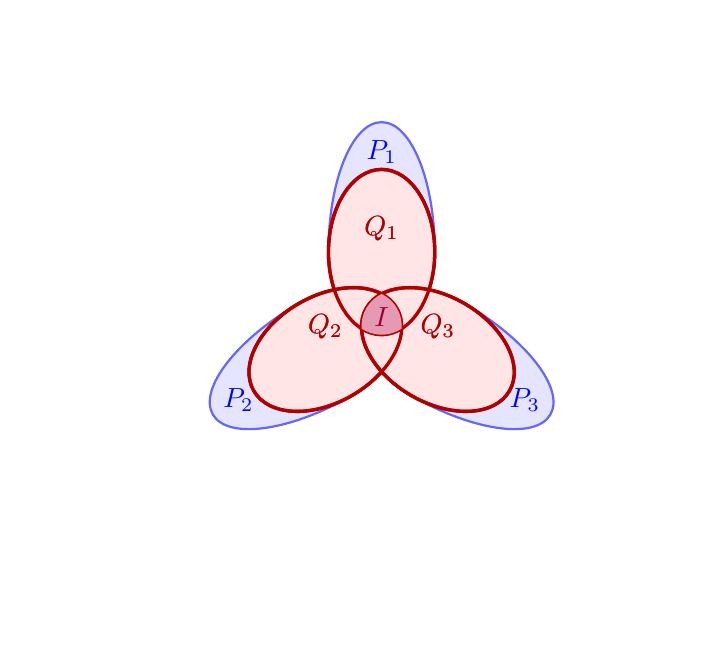
\begin{tikzpicture}[scale=0.75, thick]
  % Prime ideals (larger enclosing ellipses) clipped to show only half of the ellipse

\begin{scope}
  \clip (0,2.2) rectangle (5,6);
  \draw[blue!60, fill=blue!10] (1.5,2.2) ellipse [x radius=2.2, y radius=0.9, rotate=90];
  \node[text=blue] at (1.5, 3.9) {$P_1$};
\end{scope}

\begin{scope}[rotate around={120:(1.5,1.1)}]
  \clip (0,2.2) rectangle (5,6);
  \draw[blue!60, fill=blue!10] (1.5,2.2) ellipse [x radius=2.2, y radius=0.9, rotate=90];
  \node[text=blue] at (1.5, 3.9) {$P_2$};
\end{scope}

\begin{scope}[rotate around={240:(1.5,1.1)}]
  \clip (0,2.2) rectangle (5,6);
  \draw[blue!60, fill=blue!10] (1.5,2.2) ellipse [x radius=2.2, y radius=0.9, rotate=90];
  \node[text=blue] at (1.5, 3.9) {$P_3$};
\end{scope}

  % Primary ideals (smaller, slightly rotated ellipses)
  \draw[red!70!black, very thick,fill=red!10] (1.5,2.2) ellipse [x radius=1.4, y radius=0.9, rotate=90] node[above] {$Q_1$};

\begin{scope}[rotate around={120:(1.5,1.1)}]
  \draw[red!70!black, very thick,fill=red!10] (1.5,2.2) ellipse [x radius=1.4, y radius=0.9, rotate=90] node[above] {$Q_2$};
\end{scope}

\begin{scope}[rotate around={240:(1.5,1.1)}]
  \draw[red!70!black, very thick,fill=red!10] (1.5,2.2) ellipse [x radius=1.4, y radius=0.9, rotate=90] node[above] {$Q_3$};
\end{scope}

  % Primary ideals (smaller, slightly rotated ellipses) (no fill, to show borders)
  \draw[red!70!black, very thick] (1.5,2.2) ellipse [x radius=1.4, y radius=0.9, rotate=90] node[above] {$Q_1$};

\begin{scope}[rotate around={120:(1.5,1.1)}]
  \draw[red!70!black, very thick, save path=\savedpath] (1.5,2.2) ellipse [x radius=1.4, y radius=0.9, rotate=90] node[above] {$Q_2$};
\end{scope}

\begin{scope}[rotate around={240:(1.5,1.1)}]
  \draw[red!70!black, very thick, save path=\savedpathh] (1.5,2.2) ellipse [x radius=1.4, y radius=0.9, rotate=90] node[above] {$Q_3$};
\end{scope}

  % Intersection highlight for I (clip to smaller ellipses Q1,Q2,Q3)
  \begin{scope}
    \clip (1.5,2.2) ellipse [x radius=1.4, y radius=0.9, rotate=90];
    \clip[use path=\savedpath];
    \clip[use path=\savedpathh];
    \fill[purple!40] (-2,-1) rectangle (6,5);
  \end{scope}
  \node at (1.5,1.1) [purple!80!black] {$I$};

\end{tikzpicture}
\end{columns}
%\vspace*{-0.3in}
%\begin{itemize}
%  \item Each primary ideal has an associated prime ideal
%  \item The prime ideals in such a decomposition are unique
%\end{itemize}
\end{frame}

%----------------------------------
\begin{frame}{Classical Results}
\begin{itemize}
  \item \textbf{Lasker–Noether theorem}: Every ideal in a Noetherian ring admits a primary decomposition.
  \item Uniqueness up to radicals and associated primes.
\end{itemize}
\end{frame}

%----------------------------------
\begin{frame}{Algorithms for Ideal Factorization}
\centering
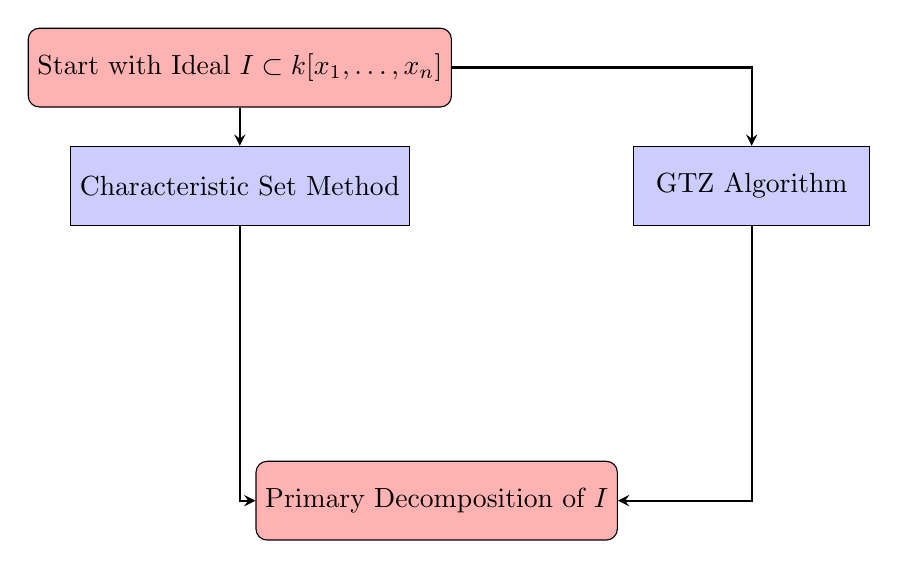
\begin{tikzpicture}[node distance=1.5cm]
\node (start) [startstop] {Start with Ideal $I \subset k[x_1,\dots,x_n]$};
\node (cs) [process, below of=start] {Characteristic Set Method};
\node (gtz) [process, right of=cs, xshift=5cm] {GTZ Algorithm};
\node (end) [startstop, below of=cs, yshift=-2.5cm, xshift=2.5cm] {Primary Decomposition of $I$};

\draw [arrow] (start) -- (cs);
\draw [arrow] (start) -| (gtz);
\draw [arrow] (cs) |- (end);
\draw [arrow] (gtz) |- (end);
\end{tikzpicture}
\end{frame}

%----------------------------------
\begin{frame}{Characteristic Set Method}
\begin{itemize}
  \item Uses elimination and triangular sets.
  \item Originates in differential algebra.
  \item Advantage: systematic structure.
  \item Limitation: ordering choice is crucial.
\end{itemize}
\end{frame}

%----------------------------------
\begin{frame}{GTZ Algorithm}
\begin{itemize}
  \item Gröbner basis-based.
  \item Splits and refines components iteratively.
  \item Widely implemented in CAS.
\end{itemize}
\centering
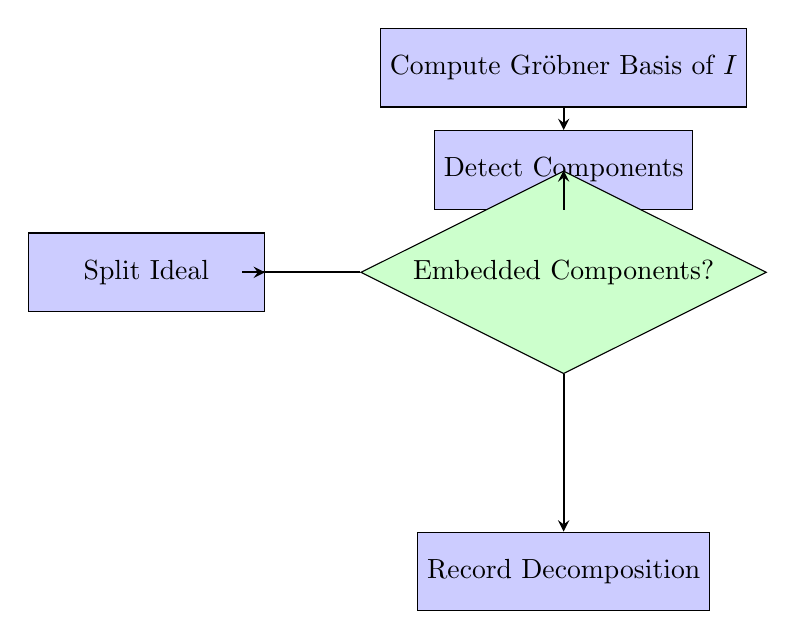
\begin{tikzpicture}[node distance=1.3cm]
\node (gb) [process] {Compute Gröbner Basis of $I$};
\node (comp) [process, below of=gb] {Detect Components};
\node (split) [decision, below of=comp] {Embedded Components?};
\node (splityes) [process, left of=split, xshift=-4cm] {Split Ideal};
\node (no) [process, below of=split, yshift=-2.5cm] {Record Decomposition};

\draw [arrow] (gb) -- (comp);
\draw [arrow] (comp) -- (split);
\draw [arrow] (split.west) -- ++(-1.5,0) -- (splityes.east);
\draw [arrow] (split.south) -- ++(0,-1) -- (no.north);
\end{tikzpicture}
\end{frame}

%----------------------------------
\begin{frame}{Worked Example 1}
\begin{itemize}
  \item Example: $I = \langle x^2-y, \, xy \rangle \subset k[x,y]$
  \item Gröbner basis computation $\rightarrow$ decomposition.
  \item Interpreted geometrically as simpler varieties.
\end{itemize}
\centering
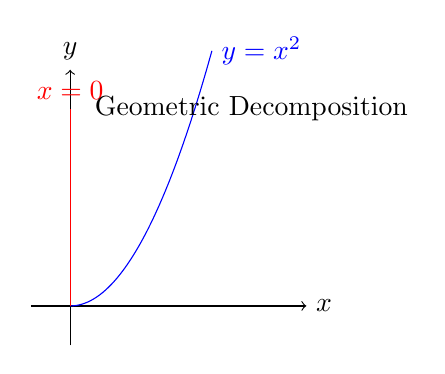
\begin{tikzpicture}
  \draw[->] (-0.5,0) -- (3,0) node[right] {$x$};
  \draw[->] (0,-0.5) -- (0,3) node[above] {$y$};
  \draw[domain=0:1.8,smooth,variable=\x,blue] plot ({\x},{\x*\x}) node[right] {$y=x^2$};
  \draw[red] (0,0) -- (0,2.5) node[above] {$x=0$};
  \node at (2.3,2.5) {Geometric Decomposition};
\end{tikzpicture}
\end{frame}

%----------------------------------
\begin{frame}{Applications to Polynomial Equations}
\begin{itemize}
  \item Decomposition $\Leftrightarrow$ splitting solution sets.
  \item Ideal $\cap$ decomposition $\Rightarrow$ variety union.
\end{itemize}
\centering
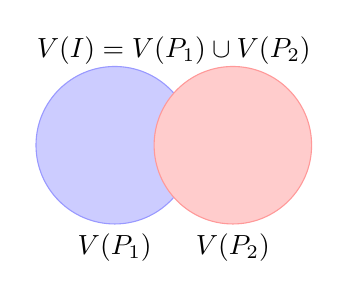
\begin{tikzpicture}
  \draw[blue!40,fill=blue!20] (0,0) circle(1);
  \draw[red!40,fill=red!20] (1.5,0) circle(1);
  \node at (0,-1.3) {$V(P_1)$};
  \node at (1.5,-1.3) {$V(P_2)$};
  \node at (0.75,1.2) {$V(I)=V(P_1)\cup V(P_2)$};
\end{tikzpicture}
\end{frame}

%----------------------------------
\begin{frame}{Applications to Differential Equations}
\begin{itemize}
  \item Characteristic set methods connect differential systems with ideals.
  \item Decomposition splits families of solutions.
\end{itemize}
\end{frame}

%----------------------------------
\begin{frame}{Current Limits and Open Problems}
\begin{itemize}
  \item Complexity is often exponential.
  \item Gröbner basis can be costly.
  \item Future directions:
    \begin{itemize}
      \item Hybrid and numerical-symbolic methods.
      \item Parallelization.
    \end{itemize}
\end{itemize}
\end{frame}

\begin{frame}
\frametitle{The New Pseudo-Solution to Hydrogen}

\[ - \frac{1}{2} \nabla^2 \Psi - \frac{1}{r} \Psi = 0 \]

\[ \Psi(x,y,z) = J_0(2\sqrt{x+r}) \]

\vskip 0.5in

$J_0$ is the Bessel function $J_0$

\end{frame}

\begin{frame}
\frametitle{Verification with Mathematica}
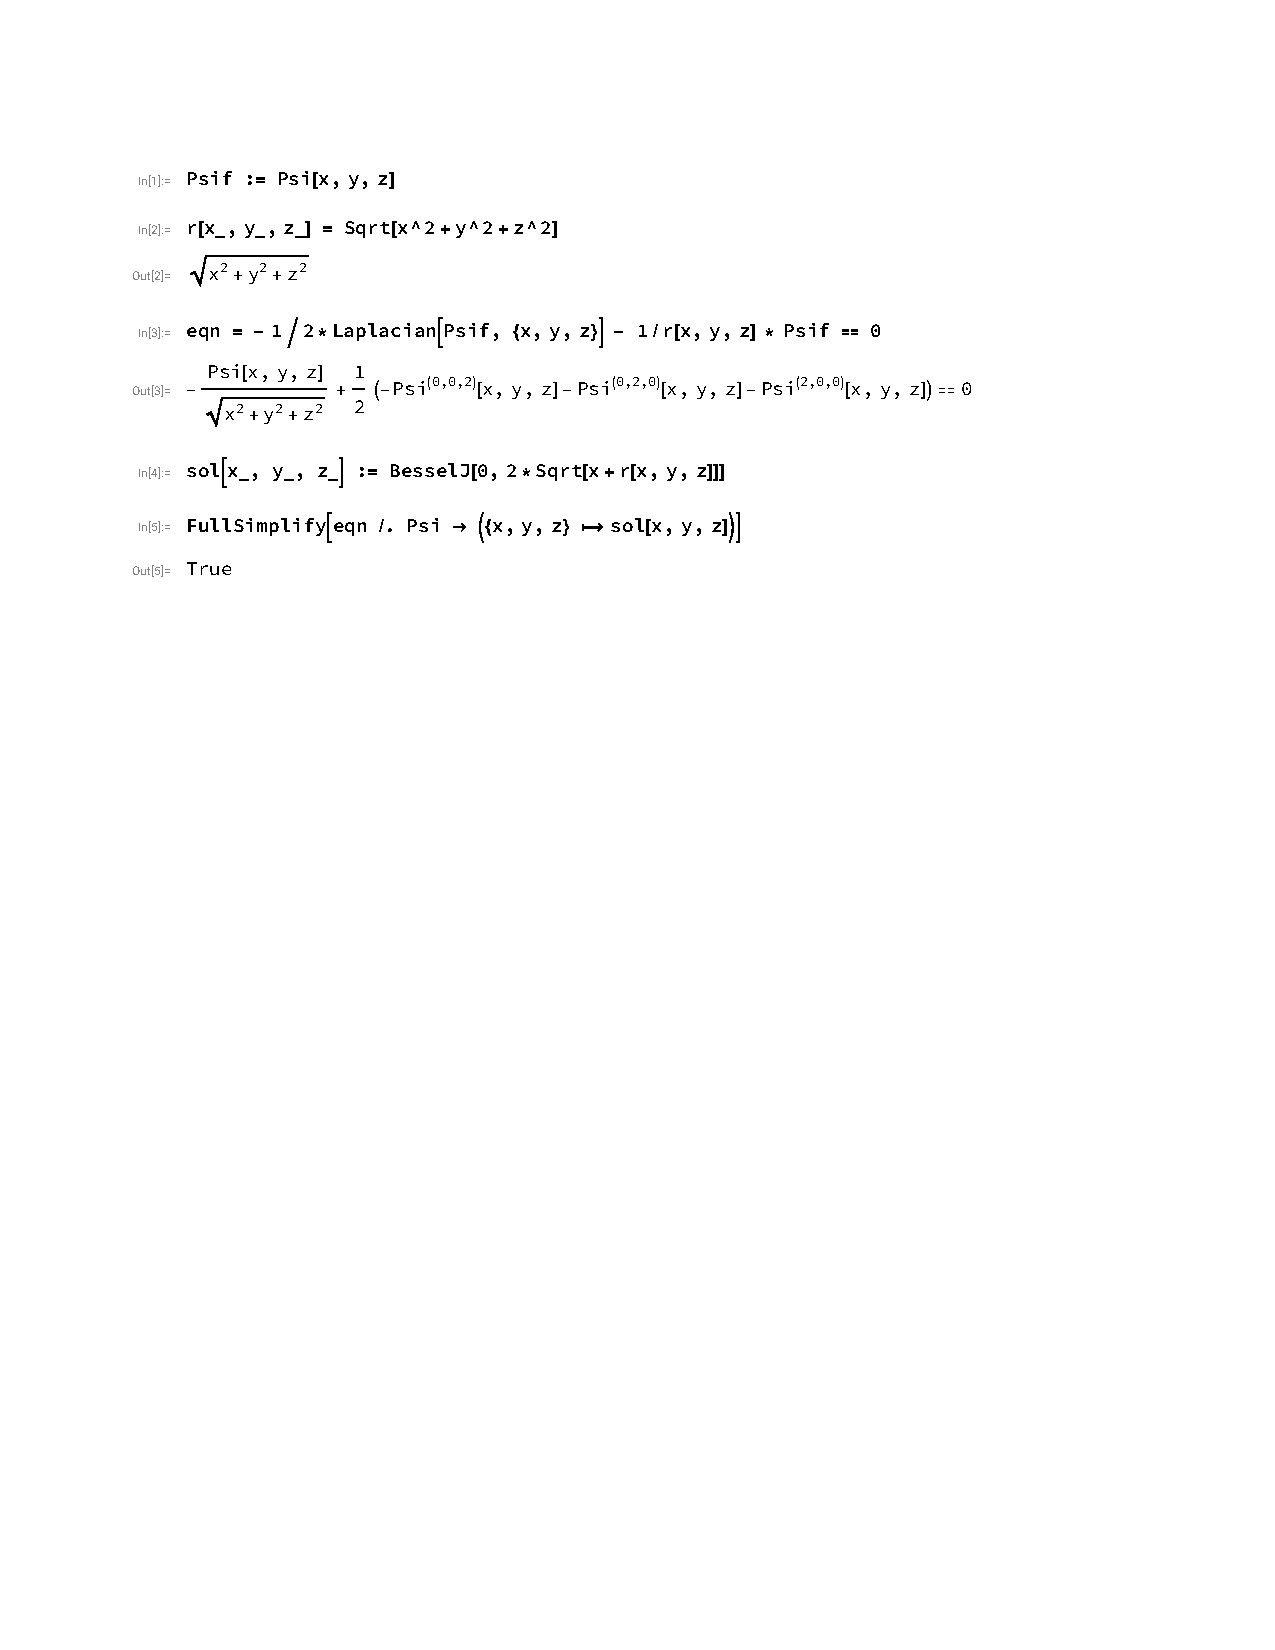
\includegraphics[page=1, clip, trim=1in 7in 1in 1in, width=\textwidth]{improved.pdf}
\end{frame}

\begin{frame}
\frametitle{The System of Equations}
%%\scriptsize
\fontsize{9}{11}\selectfont
\begin{minipage}{.7\linewidth}
\begin{equation*}
\begin{array}{r}
-2 \, c_{1} v_{0}^{3} - 4 \, c_{1} v_{0} v_{1}^{2} - 4 \, c_{1} v_{0} v_{2}^{2} - 2 \, c_{1} v_{0} v_{3}^{2} - 4 \, E a_{1} v_{0} =0\\
-2 \, c_{1} v_{0}^{3} - 4 \, c_{1} v_{0} v_{1}^{2} - 2 \, c_{1} v_{0} v_{2}^{2} - 4 \, c_{1} v_{0} v_{3}^{2} - 4 \, E a_{1} v_{0} =0\\
-2 \, c_{1} v_{0}^{3} - 2 \, c_{1} v_{0} v_{1}^{2} - 4 \, c_{1} v_{0} v_{2}^{2} - 4 \, c_{1} v_{0} v_{3}^{2} - 4 \, E a_{1} v_{0} =0\\
-3 \, b_{1} v_{0}^{2} v_{1} -  \, b_{1} v_{1}^{3} -  \, b_{1} v_{1} v_{2}^{2} -  \, b_{1} v_{1} v_{3}^{2} =0\\
-3 \, b_{1} v_{0}^{2} v_{2} -  \, b_{1} v_{1}^{2} v_{2} -  \, b_{1} v_{2}^{3} -  \, b_{1} v_{2} v_{3}^{2} =0\\
-3 \, b_{1} v_{0}^{2} v_{3} -  \, b_{1} v_{1}^{2} v_{3} -  \, b_{1} v_{2}^{2} v_{3} -  \, b_{1} v_{3}^{3} =0\\
-2 \, b_{1} v_{0}^{3} - 4 \, b_{1} v_{0} v_{1}^{2} - 4 \, b_{1} v_{0} v_{2}^{2} - 2 \, b_{1} v_{0} v_{3}^{2} =0\\
-2 \, b_{1} v_{0}^{3} - 4 \, b_{1} v_{0} v_{1}^{2} - 2 \, b_{1} v_{0} v_{2}^{2} - 4 \, b_{1} v_{0} v_{3}^{2} =0\\
-3 \, c_{1} v_{0}^{2} v_{1} -  \, c_{1} v_{1}^{3} -  \, c_{1} v_{1} v_{2}^{2} -  \, c_{1} v_{1} v_{3}^{2} - 2 \, E a_{1} v_{1} =0\\
-3 \, c_{1} v_{0}^{2} v_{2} -  \, c_{1} v_{1}^{2} v_{2} -  \, c_{1} v_{2}^{3} -  \, c_{1} v_{2} v_{3}^{2} - 2 \, E a_{1} v_{2} =0\\
-3 \, c_{1} v_{0}^{2} v_{3} -  \, c_{1} v_{1}^{2} v_{3} -  \, c_{1} v_{2}^{2} v_{3} -  \, c_{1} v_{3}^{3} - 2 \, E a_{1} v_{3} =0\\
-2 \, b_{1} v_{0}^{3} - 2 \, b_{1} v_{0} v_{1}^{2} - 4 \, b_{1} v_{0} v_{2}^{2} - 4 \, b_{1} v_{0} v_{3}^{2} =0\\
- \, c_{0} v_{0}^{2} -  \, c_{0} v_{1}^{2} -  \, c_{0} v_{2}^{2} -  \, c_{0} v_{3}^{2} - 2 \, E a_{0} - 2 \, a_{1} v_{0} =0\\
- \, c_{1} v_{0}^{3} - 3 \, c_{1} v_{0} v_{1}^{2} -  \, c_{1} v_{0} v_{2}^{2} -  \, c_{1} v_{0} v_{3}^{2} - 2 \, E a_{1} v_{0} =0\\
- \, c_{1} v_{0}^{3} -  \, c_{1} v_{0} v_{1}^{2} - 3 \, c_{1} v_{0} v_{2}^{2} -  \, c_{1} v_{0} v_{3}^{2} - 2 \, E a_{1} v_{0} =0\\
- \, c_{1} v_{0}^{3} -  \, c_{1} v_{0} v_{1}^{2} -  \, c_{1} v_{0} v_{2}^{2} - 3 \, c_{1} v_{0} v_{3}^{2} - 2 \, E a_{1} v_{0} =0\\
-2 \, a_{1} v_{0}^{2} -  \, b_{0} v_{0}^{2} -  \, b_{0} v_{1}^{2} -  \, b_{0} v_{2}^{2} -  \, b_{0} v_{3}^{2} =0\\
- \, b_{1} v_{0}^{3} - 3 \, b_{1} v_{0} v_{1}^{2} -  \, b_{1} v_{0} v_{2}^{2} -  \, b_{1} v_{0} v_{3}^{2} =0\\
- \, b_{1} v_{0}^{3} -  \, b_{1} v_{0} v_{1}^{2} - 3 \, b_{1} v_{0} v_{2}^{2} -  \, b_{1} v_{0} v_{3}^{2} =0\\
- \, b_{1} v_{0}^{3} -  \, b_{1} v_{0} v_{1}^{2} -  \, b_{1} v_{0} v_{2}^{2} - 3 \, b_{1} v_{0} v_{3}^{2} =0
\end{array}
\end{equation*}
\end{minipage}%
\begin{minipage}{.3\linewidth}
\begin{equation*}
\begin{array}{r}
-4 \, b_{1} v_{0} v_{1} v_{2} =0\\
-4 \, b_{1} v_{0} v_{1} v_{3} =0\\
-4 \, b_{1} v_{0} v_{2} v_{3} =0\\
-4 \, c_{1} v_{0} v_{1} v_{2} =0\\
-4 \, c_{1} v_{0} v_{1} v_{3} =0\\
-4 \, c_{1} v_{0} v_{2} v_{3} =0\\
-2 \, c_{0} v_{0} v_{1} - 2 \, a_{1} v_{1} =0\\
-2 \, c_{0} v_{0} v_{2} - 2 \, a_{1} v_{2} =0\\
-2 \, c_{0} v_{0} v_{3} - 2 \, a_{1} v_{3} =0\\
-2 \, a_{1} v_{0} v_{1} - 2 \, b_{0} v_{0} v_{1} =0\\
-2 \, a_{1} v_{0} v_{2} - 2 \, b_{0} v_{0} v_{2} =0\\
-2 \, a_{1} v_{0} v_{3} - 2 \, b_{0} v_{0} v_{3} =0\\
-2 \, a_{0} =0\\
-2 \, a_{0} v_{0} =0\\
\end{array}
\end{equation*}
\end{minipage}
\end{frame}

\begin{frame}[fragile]
\frametitle{The Prime Decomposition of the System of Equations}
{\tiny\begin{verbatim}
sage: I = ideal(eqns_RQQ)
sage: I.radical().primary_decomposition()
[Ideal (c1, b1, a1 - b0, a0, E, v0*c0 - b0, v0^2 - v1^2 - v2^2 - v3^2, v1^2*c0 + v2^2*c0 + v3^2*c0 - v0*b0) of Multivariate Polynomial Ring in E, v0, v1, v2, v3, a0, a1, b0, b1, c0, c1 over Rational Field,
 Ideal (b1, 2*a1 - b0, a0, v3, v2, v1, v0*c0 - b0, E*c0 - v0*c1, v0^2*c1 - E*b0) of Multivariate Polynomial Ring in E, v0, v1, v2, v3, a0, a1, b0, b1, c0, c1 over Rational Field,
 Ideal (a1, a0, v0, v1^2 + v2^2 + v3^2) of Multivariate Polynomial Ring in E, v0, v1, v2, v3, a0, a1, b0, b1, c0, c1 over Rational Field,
 Ideal (a0, v3, v2, v1, v0) of Multivariate Polynomial Ring in E, v0, v1, v2, v3, a0, a1, b0, b1, c0, c1 over Rational Field,
 Ideal (c1, c0, b1, b0, a1, a0) of Multivariate Polynomial Ring in E, v0, v1, v2, v3, a0, a1, b0, b1, c0, c1 over Rational Field]
\end{verbatim}}

\vskip -12pt
\begin{subequations}
\label{ideal}
\begin{align}
& \left(c_{1}, c_{0}, b_{1}, b_{0}, a_{1}, a_{0}\right)\label{ideal:5} \\
& \qquad \text{sets all coefficients of the ODE to zero} \nonumber \\
& \left(v_{3}, v_{2}, v_{1}, v_{0}, a_{0}\right)\label{ideal:4}\\
& \qquad \text{sets the variable $v$ to zero} \nonumber \\
& \left(v_{1}^{2} + v_{2}^{2} + v_{3}^{2}, v_{0}, a_{1}, a_{0}\right)\label{ideal:3}\\
& \qquad \text{sets the coefficient of $\Psi_{vv}$ in the ODE to zero} \nonumber \\
%% (b1, 2*a1 + b0, a0, v3, v2, v1, v0*c0 - b0, E*c0 - v0*c1, v0^2*c1 - E*b0)
& \left(v_{3}, v_{2}, v_{1}, b_{1}, c_{0} v_{0} - b_{0}, 2 a_{1} - b_{0}, a_{0}, E c_{0} - c_{1} v_{0}, v_0^2 c_1 - E b_0\right)\label{ideal:2}\\
& \qquad \text{the classical solution} \nonumber \\
& \left(v_{0}^{2} - v_{1}^{2} - v_{2}^{2} - v_{3}^{2}, c_{1}, b_{1}, b_{0} - c_{0} v_{0}, a_{1} + c_{0} v_{0}, a_{0}, E\right)\label{ideal:1}\\
& \qquad \text{the new pseudo-solution} \nonumber
\end{align}
\end{subequations}
\end{frame}

\begin{frame}
\frametitle{Shimoyama and Yokoyama Algorithm}
% left bottom right top
\includegraphics[page=9, clip, trim=1.3in 4in 0in 5.1in, scale=0.9]{1-s2.0-S0747717196900528-main.pdf}

\vfill
\small
\begin{tabular}{ll}
Source: & Takeshi Shimoyama and Kazuhiro Yokoyama, \\
        & {\it Localization and Primary Decomposition of Polynomial Ideals}, \\
        & J. Symbolic Computation (1996) {\bf 22}, 247–277 \\
\end{tabular}
\end{frame}

\begin{frame}
\frametitle{A Simple Irreducible Decomposition}

Consider this system of equations:
\[ xz = 0 \qquad yz = 0 \]

The Prime Decomposition of the Ideal

\[ (xz,yz) = (x,y) \cap (z) \]

The corresponding irreducible varieties

\begin{itemize}
\item The $x-y$ plane
\item The $z$ axis
\end{itemize}

\begin{center}

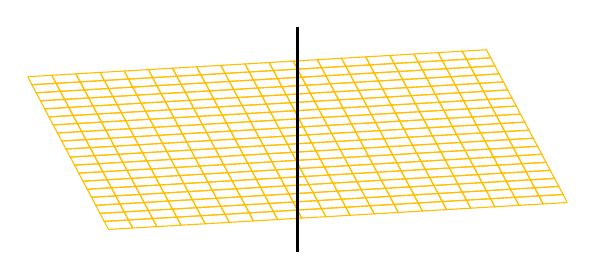
\begin{tikzpicture}
\begin{axis}[
    hide axis,
    view={10}{-30},
    samples=20
]
\addplot3 [
    mesh,
    domain=-10:10,
    y domain=-10:10,
] (
    x, y, 0
);

\pgfmathsetmacro\slice{.4}

\addplot3 [
    mesh,
    domain=-10:10,
    color=black,
    line width=1pt,
] (
    0, 0, x
);

\end{axis}
\end{tikzpicture}
\end{center}
\end{frame}

\begin{frame}[t]
\frametitle{Independent Sets}
\begin{definition}[Independent set]
Let $I$ be an ideal of the polynomial ring $Q[X]$. A subset $U$ in $X$ is called an {\it independent
set} modulo $I$ if $I \cap Q[U] = \{0\}$.

%An independent set U modulo I is called a maximally
%independent set modulo I if I ∩ Q[U ∪ {x}] 6= {0} for every variable x in X \ U .
%A subset U in X is called a strongly independent set modulo I with respect to an
%admissible order < if HT (I) ∩ T (U ) = ∅, where T (U ) is the set of all terms in U
%and HT (I) is the set of head terms of all non-zero elements in I with respect to <.
%Moreover, U is called a maximal strongly independent set modulo I with respect to <
%if U is a strongly independent set and HT (I) ∩ T (U ∪ {x}) 6= ∅ for every variable x
%in X \ U .
\end{definition}

\begin{definition}[Maximally Independent set]
An independent set $U \mod I$ is called a {\it maximally
independent set} modulo $I$ if $I \cap Q[U \cup {x}] \ne \{0\}$ for every variable $x$ in $X \backslash U$.
%A subset U in X is called a strongly independent set modulo I with respect to an
%admissible order < if HT (I) ∩ T (U ) = ∅, where T (U ) is the set of all terms in U
%and HT (I) is the set of head terms of all non-zero elements in I with respect to <.
%Moreover, U is called a maximal strongly independent set modulo I with respect to <
%if U is a strongly independent set and HT (I) ∩ T (U ∪ {x}) 6= ∅ for every variable x
%in X \ U .
\end{definition}

\vfill

\begin{tabular}{ll}
Source: & Definition A.9 \\
        & Takeshi Shimoyama and Kazuhiro Yokoyama, \\
        & {\it Localization and Primary Decomposition of Polynomial Ideals}, \\
        & J. Symbolic Computation (1996) {\bf 22}, 247–277 \\
\end{tabular}
\end{frame}

\begin{frame}
\frametitle{Independent Sets}
\begin{example}
Consider the ideal $(xz,yz)$ in $Q[x,y,z]$

\begin{align*}
(xz,yz) \cap Q[x] &= \{0\} &{\rm IS} \\
(xz,yz) \cap Q[y] &= \{0\} &{\rm IS} \\
(xz,yz) \cap Q[z] &= \{0\} &{\rm MIS} \\
\\
(xz,yz) \cap Q[x,y] &= \{0\} &{\rm MIS} \\
(xz,yz) \cap Q[x,z] &= (xz) \\
(xz,yz) \cap Q[y,z] &= (yz) \\
\\
(xz,yz) \cap Q[x,y,z] &= (xz,yz) \\
\end{align*}
\end{example}

\end{frame}

\begin{frame}
\frametitle{Independent Sets}
\begin{example}[cont]
Continuing with the ideal $(xz,yz)$ in $Q[x,y,z]$.

\vskip 12pt

$\{z\}$ is a MIS, so let's move it into the coefficient field:

\vskip 12pt

In $Q(z)[x,y]$, $(xz,yz) = (x,y)$.

\vskip 12pt

$(x,y)$ is one of our irreducible components.

\vskip 12pt

Likewise, let's use $\{x,y\}$ as our MIS, and move it into the coefficient field:

\vskip 12pt

In $Q(x,y)[z]$, $(xz,yz) = (z)$.

\vskip 12pt

$(z)$ is our other irreducible component.

\end{example}

\end{frame}

\begin{frame}
\frametitle{Monomial Orders}
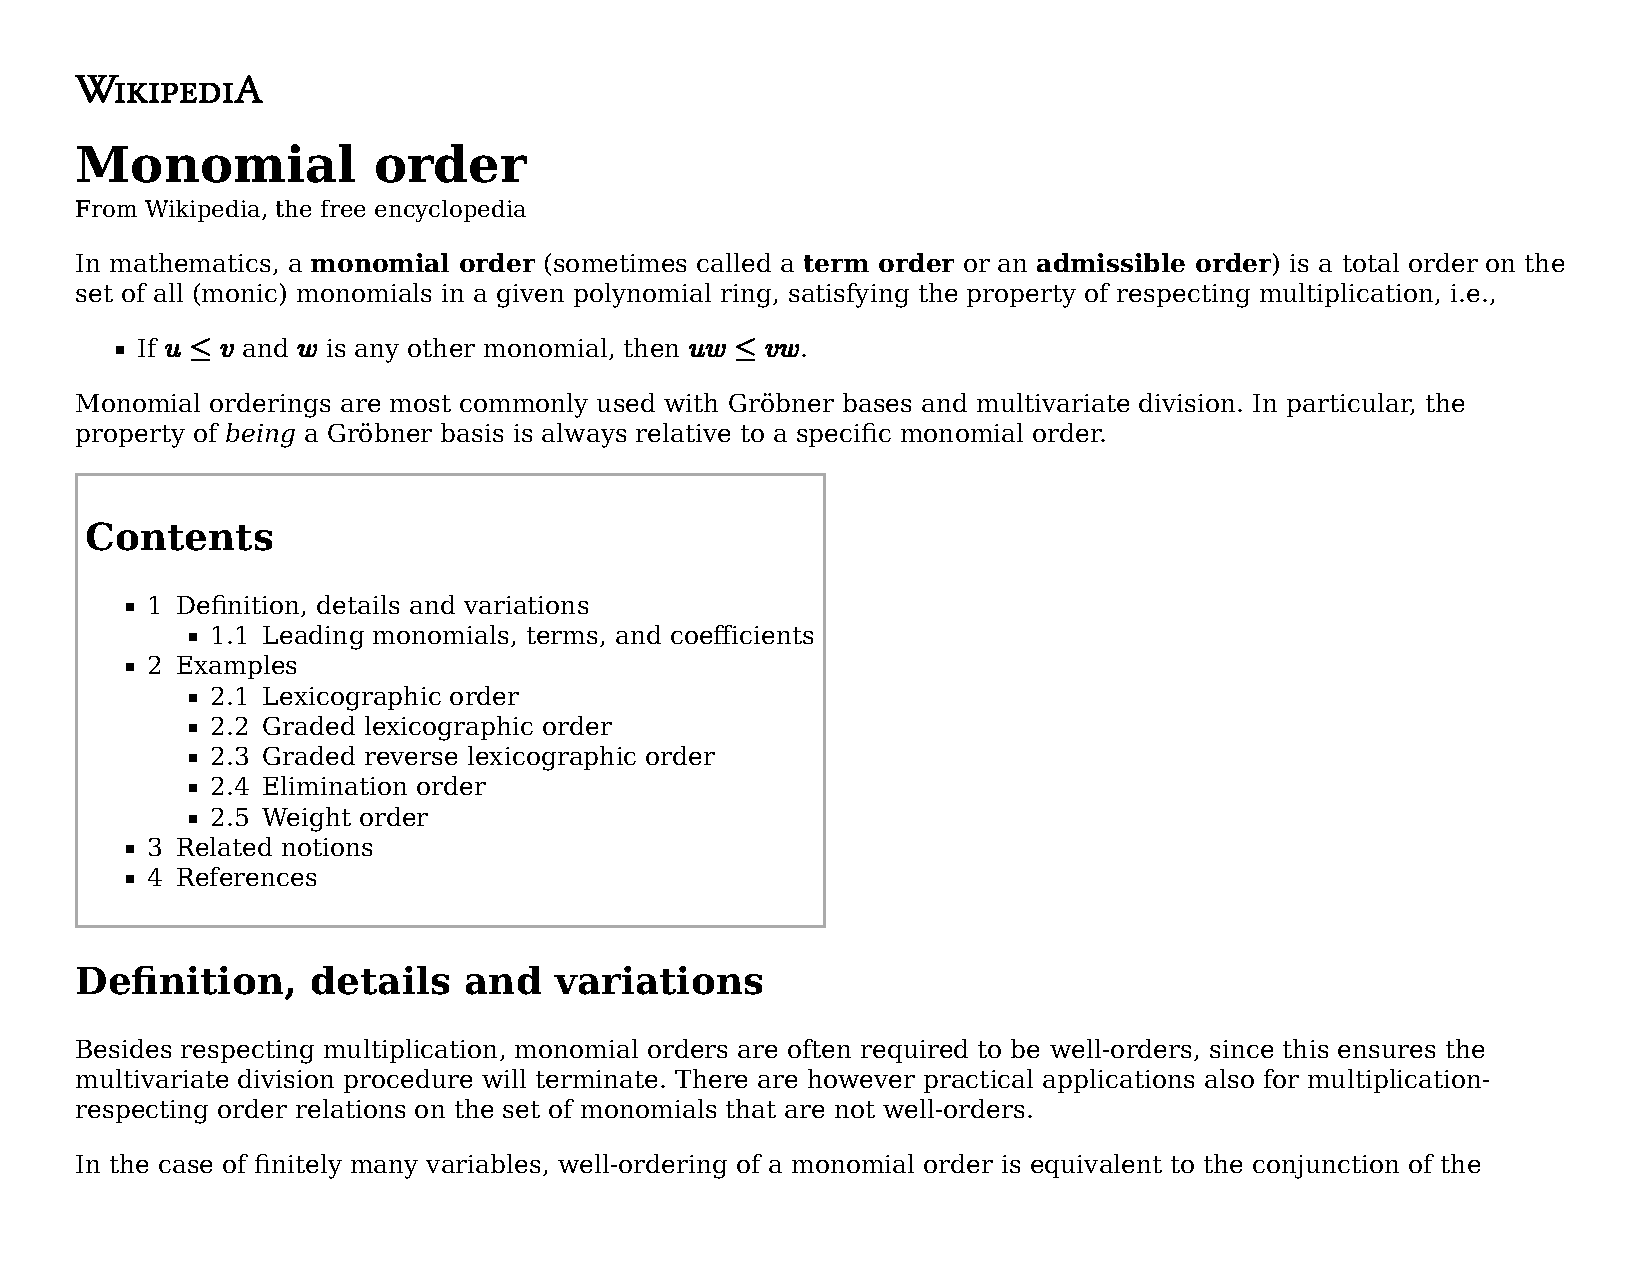
\includegraphics[page=1, clip, trim=0in 5.5in 0in 0in, width=\textwidth]{Monomial order - Wikipedia.pdf}
\vskip 20pt
{\bf Examples of Monomial Orders} (all with $x>y>z$)
\begin{itemize}
\item Lexicographic

$\qquad x^4 > x^3y > x^3 > x^2y^4 > x > y^3$
\item Graded Lexicographic

$\qquad x^2y^4 > x^4 > x^3y > x^3 > y^3 > x$

$\qquad x^2 > xy > xz > y^2 > yz > z^2$
\item Graded Reverse Lexicographic (often the fastest computationally)

$\qquad x^2 > xy > y^2 > xz > yz > z^2$
\end{itemize}
\end{frame}

\begin{frame}
\frametitle{Cox, Little, O'Shea

{\it Ideals, Varieties, and Algorithms} (4th ed)}
\includegraphics[page=22, clip, trim=0in 0.9in 0in 7in, width=\textwidth]{IVA.pdf}
\includegraphics[page=23, clip, trim=0in 7.9in 0in 0.7in, width=\textwidth]{IVA.pdf}
\hrule
\includegraphics[page=46, clip, trim=0in 5.2in 0in 2.5in, width=\textwidth]{IVA.pdf}
\end{frame}

\begin{frame}
\frametitle{Gr\"obner Bases}
\begin{definition}[Gr\"obner Basis]
Given a ring with a specified monomial order,
a {\it Gr\"obner Basis} or {\it standard basis} for an ideal $I$ is a set of
polynomials $G$ such that:
\begin{enumerate}
\item The polynomials in $G$ form a basis for the ideal $I$
\item The leading terms in $G$ form a basis for the ideal ${\rm lt}(I)$ formed by the leading terms in $I$.
\end{enumerate}
\end{definition}

\begin{example}
In the ring ${\mathbb Z}[x,y,z]$ with lexicographic ordering $x>y>z$, the ideal $(2x+3y+4z-5, 3x+4y+5z-2)$
has a reduced Gr\"obner basis given by
\begin{align*}
2x-2z+28 \\
3x-3z+42 \\
y+2z-11
\end{align*}
\end{example}
\end{frame}

\begin{frame}
\frametitle{GPT-5's Comparison of polynomial solution methods}
\tiny
\begin{table}[h!]
\centering
\renewcommand{\arraystretch}{1.4}
\begin{tabular}{|p{2.3cm}|p{2cm}|p{2cm}|p{2.5cm}|}
\hline
\textbf{Feature} & \textbf{Characteristic Sets (Wu’s Method)} & \textbf{Gröbner Bases} & \textbf{Regular Chains / Triangular Decomposition} \\
\hline
\textbf{Output form} & Triangular set (distinct main variable per polynomial) & Canonical Gröbner basis for chosen monomial order & Triangular sets with associated inequations \\
\hline
\textbf{Dependence on ordering} & Strongly dependent on variable ranking & Canonical once order is fixed & Depends on chosen variable order \\
\hline
\textbf{Uniqueness} & Not unique (varies with ranking) & Unique (for fixed monomial order) & Not unique \\
\hline
\textbf{Ease of solving} & Procedural: solve one variable at a time & Requires back-substitution, not directly triangular & Procedural like characteristic sets, but more refined \\
\hline
\textbf{Handling of inequations / branches} & Case distinctions may be needed during pseudo-division & Purely equations (ideal-based) & Explicit handling of inequations and case splits \\
\hline
\textbf{Algebraic guarantees} & Not directly tied to irreducible decomposition or ideal theory & Deep ties to algebraic geometry (ideal membership, dimension, Hilbert series) & Connects more directly to geometric decomposition into varieties \\
\hline
\textbf{Computation cost} & Often efficient in practice (esp. in geometry theorem proving) & Can be doubly exponential in worst case & Can be heavy due to branching, but manageable in practice \\
\hline
\textbf{Best use cases} & Geometry theorem proving, structured elimination & General-purpose algebraic computation, canonical decomposition & Computing solution varieties with inequations, parametric systems \\
\hline
\end{tabular}
\caption{Comparison of methods for decomposing polynomial systems.}
\end{table}
\end{frame}

\begin{frame}
\frametitle{Flexibility in constructing Gr\"obner Bases}
Much of the utility of Gr\"obner bases lies in the flexibility in how they can be defined.
\begin{itemize}
\item Many monomial orders can be defined

Lexicographic orders can be used to eliminate specific variables

\vskip 12pt
\item Variables can be moved into the coefficient field

Maximally Independent Sets can be used to reduce to zero-dimensional ideals
\end{itemize}
\end{frame}

\begin{frame}
\frametitle{Buchberger's Algorithm}

{\bf Input:} A set of polynomials $F$ that generates $I$

{\bf Output:} A Gröbner basis $G$ for $I$

\begin{enumerate}
\item $G := F$
\item For every $f_i,f_j$ in $G$, denote by $g_i$ the leading term of $f_i$ with respect to the given monomial ordering,
and by $a_{ij}$ the least common multiple of $g_i$ and $g_j$
\item Choose two polynomials in $G$ and let $S_{ij}=\frac{a_{ij}}{g_i}f_i  - \frac{a_{ij}}{g_j}f_j $

(Note that the leading terms here will cancel by construction).
\item Reduce $S_{ij}$, with the multivariate division algorithm relative to the set $G$ until the result is not further reducible.

If the result is non-zero, add it to $G$.
\item Repeat steps 2-4 until all possible pairs are considered, including those involving the new polynomials added in step 4.
\item Output $G$
\end{enumerate}

Source: Wikipedia, {\it Buchberger's Algorithm}
\end{frame}

%----------------------------------
\begin{frame}[fragile]{Profiling Singular (data collection)}

A large polynomial system (33 variables, 3486 equations, 16,517,523 terms) over $\mathbb{F}_{536870909}$ is in {\tt helium-16.6-R536870909}

\vskip 12pt

In one window, we run the calculation:

{\tiny\begin{verbatim}
baccala@samsung:~/src/helium$ ../sage/sage
sage: import pickle
sage: with open('helium-16.6-R536870909', 'rb') as f:
....:     eqns = pickle.load(f)
....: 
sage: I = ideal(eqns)
sage: bwb = I.minimal_associated_primes()
\end{verbatim}}

In another window, we profile it:

{\tiny\begin{verbatim}
baccala@samsung:~/src/helium$ ps ax | grep sage
 148747 pts/4    S+     0:00 /bin/sh /home/baccala/src/sage/src/bin/sage-python /home/baccala/src/sage/src/bin/sage-ipython -i
 148818 pts/4    S+     0:00 /bin/sh /home/baccala/src/sage/src/bin/sage-python /home/baccala/src/sage/src/bin/sage-cleaner
 148819 pts/4    S+     0:00 python3 /home/baccala/src/sage/src/bin/sage-cleaner
 148820 pts/4    Rl+    0:51 python3 /home/baccala/src/sage/src/bin/sage-ipython -i
 148985 pts/1    S+     0:00 grep --color=auto sage
baccala@samsung:~/src/helium$ perf record --call-graph dwarf -g -p 148820 sleep 30
\end{verbatim}}
\end{frame}


%----------------------------------
\begin{frame}[fragile]{Profiling Singular (data analysis)}
\tiny\begin{verbatim}
baccala@samsung:~/src/helium$ perf report

    99.86%     0.00%  python3  libSingular-4.4.1.so                      [.] yyparse()
            |
            ---yyparse()
               iiExprArithM(sleftv*, sleftv*, int)
               iiExprArith1Tab(sleftv*, sleftv*, int, sValCmd1 const*, int, sConvertTypes const*)
               jjSTD(sleftv*, sleftv*)
               kStd_internal(sip_sideal*, sip_sideal*, tHomog, intvec**, bigintmat*, int, int, intvec*, int (*)(skStrategy*))
               bba(sip_sideal*, sip_sideal*, intvec*, bigintmat*, skStrategy*)
               |          
                --99.34%--enterpairs(spolyrec*, int, int, int, skStrategy*, int)
                          |          
                           --99.34%--initenterpairs(spolyrec*, int, int, int, skStrategy*, int)
                                     |          
                                     |--84.24%--chainCritNormal(spolyrec*, int, skStrategy*)
                                     |          |          
                                     |          |--81.56%--kMergeBintoL(skStrategy*)
                                     |          |          |          
                                     |          |           --81.40%--__memcpy_avx_unaligned_erms (inlined)
                                     |          |          
                                     |           --2.68%--deleteIfCompareChain(spolyrec*, int, skStrategy*, int (*)(spolyrec*, spolyrec*, spolyrec*, spolyrec*, ip_sring*), bool, bool, bool)
                                     |                     |          
                                     |                      --2.60%--pCompareChain(spolyrec*, spolyrec*, spolyrec*, spolyrec*, ip_sring*)
                                     |          
                                     |--13.77%--deleteIfAble(spolyrec*, skStrategy*, bool)
                                     |          |          
                                     |           --4.17%--isPairsetInL(std::reverse_iterator<__gnu_cxx::__normal_iterator<sLObject*, std::vector<sLObject, std::allocator<sLObject> > > >&, spolyrec*, spolyrec*, skStrategy*)
                                     |          
                                      --1.32%--enterOnePairNormal(int, spolyrec*, int, int, skStrategy*, int)
\end{verbatim}
\end{frame}


%----------------------------------
\begin{frame}[fragile]{A Buggy Comparator}
\tiny\begin{verbatim}
int posInL110 (const LSet set, const int length, LObject* p,const kStrategy) {
  if (length<0) return 0;

  int o = p->GetpFDeg();
  int op = set[length].GetpFDeg();
  int cmp_int= -currRing->OrdSgn;

  if ((op > o)
  || ((op == o) && (set[length].length >p->length))
  || ((op == o) && (set[length].length <= p->length) && (pLmCmp(set[length].p,p->p) != cmp_int)))
    return length+1;
  int i;
  int an = 0;
  int en= length;
  loop
  {
    if (an >= en-1)
    {
      op = set[an].GetpFDeg();
      if ((op > o)
      || ((op == o) && (set[an].length >p->length))
      || ((op == o) && (set[an].length <=p->length) && (pLmCmp(set[an].p,p->p) != cmp_int)))
        return en;
      return an;
    }
    i=(an+en) / 2;
    op = set[i].GetpFDeg();
    if ((op > o)
    || ((op == o) && (set[i].length > p->length))
    || ((op == o) && (set[i].length <= p->length) && (pLmCmp(set[i].p,p->p) != cmp_int)))
      an=i;
    else
      en=i;
  }
}
\end{verbatim}
\end{frame}

\begin{frame}{Contrasting Data Structures: Array vs. Tree}
\centering
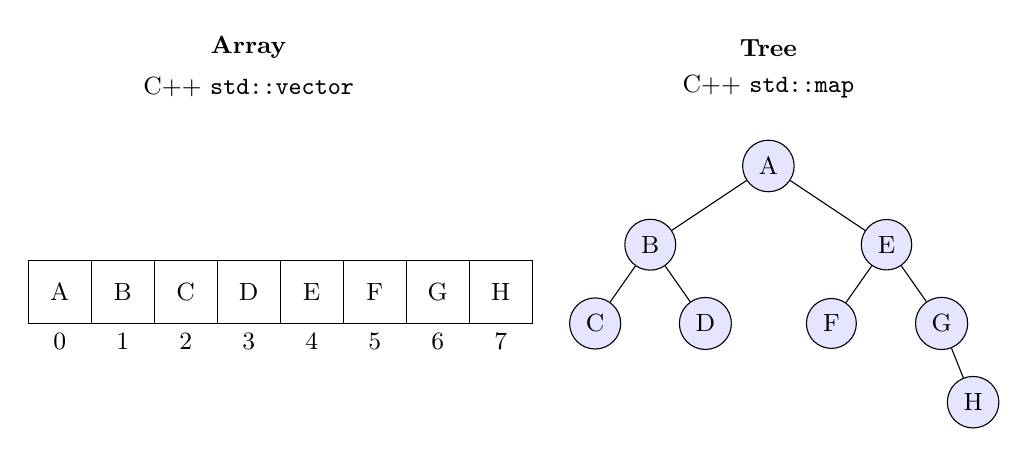
\begin{tikzpicture}[every node/.style={font=\small}]

% --- Array ---
\node at (2.8,3.5) {\textbf{Array}};
\node at (2.8,3) {C++ {\tt std::vector}};

\foreach \i/\val in {0/A,1/B,2/C,3/D,4/E,5/F,6/G,7/H} {
  \draw (0.8*\i,0) rectangle (0.8*\i+0.8,0.8);
  \node at (0.8*\i+0.4,0.4) {\val};
  \node[below] at (0.8*\i+0.4,0) {\i};
}

% --- Tree ---
\begin{scope}[shift={(-0.6,0)}]
\node at (10,3.5) {\textbf{Tree}};
\node at (10,3) {C++ {\tt std::map}};

% level 0
\node[circle,draw,fill=blue!10] (n0) at (10,2) {A};

% level 1
\node[circle,draw,fill=blue!10] (n1) at (8.5,1) {B};
\node[circle,draw,fill=blue!10] (n2) at (11.5,1) {E};

% level 2
\node[circle,draw,fill=blue!10] (n3) at (7.8,0) {C};
\node[circle,draw,fill=blue!10] (n4) at (9.2,0) {D};
\node[circle,draw,fill=blue!10] (n5) at (10.8,0) {F};
\node[circle,draw,fill=blue!10] (n6) at (12.2,0) {G};

% level 3 (just one child to make 8 total)
\node[circle,draw,fill=blue!10] (n7) at (12.6,-1) {H};

% connections
\draw (n0) -- (n1);
\draw (n0) -- (n2);
\draw (n1) -- (n3);
\draw (n1) -- (n4);
\draw (n2) -- (n5);
\draw (n2) -- (n6);
\draw (n6) -- (n7);

\end{scope}

\end{tikzpicture}
\end{frame}

\begin{frame}
\frametitle{The Rosenfeld-Gr\"obner Algorithm}
\begin{exampleblock}{Francois Boulier, Daniel Lazard, François Ollivier, Michel Petitot
Representation for the radical of a finitely generated differential ideal
}
\includegraphics[page=2, clip, trim=0in 0in 0in 5.2in, width=\textwidth]{blop.pdf}
\end{exampleblock}
\end{frame}

%----------------------------------
\begin{frame}{The Big Picture}
\small
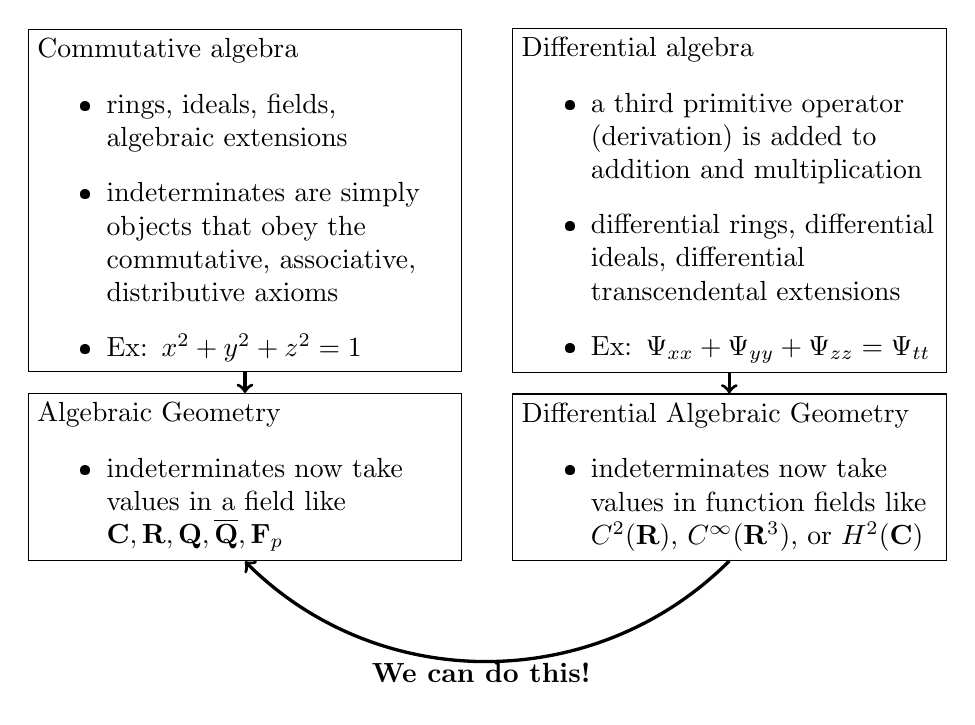
\begin{tikzpicture}[node distance=20pt]
\node (commutative algebra) [draw, text width=150pt] {Commutative algebra
      \begin{itemize}
        \item rings, ideals, fields, algebraic extensions
        \item indeterminates are simply objects that obey the commutative, associative, distributive axioms
        \item Ex: $x^2+y^2+z^2=1$
      \end{itemize}
};
\node (algebraic geometry) [draw, node distance=100pt, below of=commutative algebra, text width=150pt] {Algebraic Geometry
      \begin{itemize}
        \item indeterminates now take values in a field like $\mathbf{C}, \mathbf{R}, \mathbf{Q}, \overline{\mathbf{Q}}, \mathbf{F}_p$
      \end{itemize}
};
\node (differential algebra) [draw, node distance=175pt, right of=commutative algebra, text width=150pt] {Differential algebra
      \begin{itemize}
        \item a third primitive operator (derivation) is added to addition and multiplication
        \item differential rings, differential ideals, differential transcendental extensions
        \item Ex: $\Psi_{xx}+\Psi_{yy}+\Psi_{zz}=\Psi_{tt}$
      \end{itemize}
};
\node (differential algebraic geometry) [draw, node distance=100pt, below of=differential algebra, text width=150pt] {Differential Algebraic Geometry
      \begin{itemize}
        \item indeterminates now take values in function fields like $C^2(\mathbf{R})$,
$C^\infty(\mathbf{R}^3)$, or $H^2(\mathbf{C})$
      \end{itemize}
};

\draw [very thick, ->] (commutative algebra.south) -- (algebraic geometry.north);
\draw [very thick, ->] (differential algebra.south) -- (differential algebraic geometry.north);

\draw [very thick, ->] (differential algebraic geometry.south) to[out=-135, in=-45] (algebraic geometry.south);

\node at (3,-6) {\bf We can do this!};

\end{tikzpicture}
\end{frame}

%----------------------------------
\begin{frame}{Summary and Conclusions}
\begin{itemize}
  \item Every ideal in a Noetherian ring can be decomposed.
  \item Algorithms (Characteristic Set, GTZ) make this practical.
  \item Applications: polynomial and differential systems.
\end{itemize}
\end{frame}

%----------------------------------
\begin{frame}{Questions?}
  \centering
  \Huge Thank you! \\
  \vspace{1cm}
  \Large Questions welcome.
\end{frame}

\end{document}
